%===============================================================================
% (c) Dominik Harmim


\chapter{Introduction}

Bugs are an integral part of computer programs ever since the inception
of the programming discipline. Unfortunately, they are often hidden
in unexpected places, and they can lead to unexpected behaviour which
may cause significant damage. Nowadays there are many possible
ways of catching bugs in the development process. Dynamic analysis
tools or tools for automated testing are often used. These methods
are satisfactory in many cases. Nevertheless, they can still leave
too many bugs undetected, because they are able to analyse only
certain program flows, dependent on its input data. An alternative
solution is a~\emph{static analysis}. Of course, it has some shortages
as well. The big issue is \emph{scalability} on extensive codebases and
considerable high rate of incorrectly reported errors (so-called
\emph{false positives}, also called \emph{false alarms}).

Not long ago, Facebook introduced \emph{Facebook Infer}\,--\,a~tool for
creating \emph{highly scalable} \emph{compositional}, \emph{incremental},
and \emph{interprocedural} static analysers. Facebook Infer is a~live tool
and it is still under the development. Anyway, it is in everyday use in
Facebook itself, Spotify, Uber, Mozilla, WhatsApp and other well-known
companies. Currently, Facebook Infer provides several analysers implemented
as modules in the whole framework. These analysers check for various types
of bugs, e.g., buffer overflows, thread-safety, null-dereferencing, or
memory leaks. Facebook Infer also aims to create a~framework for building
new analysers quickly and easily. The current version of Facebook Infer still
misses better support for \emph{concurrency} bugs. While it provides a~fairly
advanced \emph{data race} analyser, it is limited to Java programs only and
fails for C~programs, which require more through manipulation with locks.

In \emph{concurrent programs}, there are often \emph{atomicity requirements}
for execution of specific sequences of instructions. Violating these
requirements may cause many kinds of problems, such as unexpected
behaviour, exceptions, segmentation faults, or other failures.
\emph{Atomicity violations} are usually not verified by compilers,
unlike syntactic or some sorts of semantic rules. Atomicity requirements,
in most cases, are not even documented. It means that typically only
programmers must take care of following these requirements. In general,
it is very difficult to avoid errors in \emph{atomicity-dependent
programs}, especially in large projects, and even harder and time-consuming
is finding and fixing these errors.

In this thesis, there is described proposal, implementation, and experimental
verification and evaluation of \emph{Atomer}\,---\,static analyser for
finding atomicity violations\,---\,which is implemented as an extension for
Facebook Infer. In particular, the concentration is put on an
\emph{atomic execution of sequences of function calls}, which is often
required, e.g., when using certain library calls. The implementation targets
to C/C++ programs that use \emph{PThreads} locks.

The development of \emph{Atomer} has been discussed with developers of
Facebook Infer, and it is a~part of the H2020 ECSEL project Aquas. Parts
of this paper are taken over~\cite{excel2019FBInfer}, which I~wrote
together with Vladimír Marcin and Ondřej Pavela. In~\cite{excel2019FBInfer},
there were presented preliminary results of my thesis.

The rest of the paper is organised as follows. In
Chapter~\ref{chap:preliminaries}, there are described all the topics
which are necessary to understand before reading the rest of the paper. In
particular, Section~\ref{sec:staticAnalysisAI} deals with
a~\emph{static analysis} based on \emph{abstract interpretation}.
Facebook Infer, which uses abstract interpretation, is described in
Section~\ref{sec:fbinfer}. And in Section~\ref{sec:contracts}, there is
described the concept of \emph{contracts for concurrency}. Proposal of a~static
analyser for detection \emph{atomicity violations}, based on this concept, is
described in Chapter~\ref{chap:proposal}. Its implementation is in
Chapter~\ref{chap:implementation} and experimental results are presented
in Chapter~\ref{chap:experiments}. Finally, Chapter~\ref{chap:conclusion}
concludes the paper. Appendix~\ref{chap:memoryMedia} lists contents
of attached memory media and Appendix~\ref{chap:manual} serves as an
installation and user manual.



\chapter{Preliminaries}
\label{chap:preliminaries}

This chapter explains the theoretical background on which stands the
thesis. It also explains and describes the existing tools used in the
thesis. Lastly, the chapter deals with principles which this thesis
got inspired by.

The aim of this thesis is to propose a~\emph{static analyser} and implement
it in \emph{Facebook Infer}. So, in Section~\ref{sec:staticAnalysisAI},
there is a~brief explanation of a~\emph{static analysis} itself, and then an
explanation of \emph{abstract interpretation} that is used in Facebook Infer.
Facebook Infer, its principles and features illustrate
Section~\ref{sec:fbinfer}. The proposal of a~solution is based on the
concept of \emph{contracts for concurrency}, which is discussed and defined
in Section~\ref{sec:contracts}.


\section{Static Analysis by Abstract Interpretation}
\label{sec:staticAnalysisAI}

According to~\cite{staticAnalysisMoller}, a~\emph{static analysis} of
programs is reasoning about the behaviour of computer programs without
actually executing them. It has been used since the 1970s for optimising
compilers for generating effective code. More recently, it has proven
valuable also for automatic error detection, verification tools and it
is used in other tools that can help programmers. Intuitively,
a~static program analyser is a~program that reasons about the behaviour
of other programs, in other words, a~static program analyser checks if the
\emph{program semantics} of a~given program fulfils the given
\emph{specification}, as illustrates Figure~\ref{fig:staticAnalysis}
\cite{AIBasedFormalMethodsCousot}. Nowadays, a~static analysis is one of
the fundamental concepts of \emph{formal verification}. It aims to
automatically answer questions about a~given program, such as
e.g.~\cite{staticAnalysisMoller}:
\begin{itemize}
    \item
        \textbf{Are certain operations executed \emph{atomically}?}

    \item
        Does the program terminate on every input?

    \item
        Can the program \emph{deadlock}?

    \item
        Does there exist an input that leads to a~\emph{null-pointer
        dereference}, a~\emph{division-by-zero}, or an \emph{arithmetic
        overflow}?

    \item
        Are all variable initialised before they are used?

    \item
        Are arrays always accessed within their bound?

    \item
        Does the program contain \emph{dead code}?

    \item
        Are all resources correctly released after their last
        use?
\end{itemize}

\begin{figure}[hbt]
    \centering
    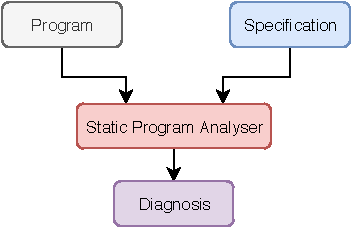
\includegraphics[width=.4 \linewidth]{static_analysis.pdf}
    \caption{
        A~static program analysis~\cite{AIBasedFormalMethodsCousot}
    }
    \label{fig:staticAnalysis}
\end{figure}

It is well-known that testing, i.e., executing programs
with some input data and examining the output, may expose errors, but it
can not prove their absence. (It was also famously stated by Edsger W.
Dijkstra: \uv{\textit{Program testing can be used to show the presence of bugs,
but never to show their absence!}}.) However, a~static program analysis
can prove their absence\,---\,with some \emph{approximation}\,---\,it can
check \emph{all possible executions} of the programs and provide guarantees
about their properties. Another advantage of a~static analysis is that the
analysis can be performed during the development process, so the program
does not have to be executable yet and it already can be analysed.
The significant issue is how to ensure high precision and
\emph{scalability} to be useful in practice. The biggest disadvantage is
that a~static analysis can produce many \emph{false alarms}\footnote{
\textbf{False alarms}\,--\,incorrectly reported an error. Also called
\emph{false positives}.}, but it is often
resolved by accepting \emph{unsoundness}\footnote{\textbf{Soundness}\,--\,if
a~verification method claims that a~system is correct according to a~given
specification, it is truly correct.~\cite{favStaticAnalysis}}.

Various forms of a~static analysis of programs have been invented, for
instance~\cite{favStaticAnalysis}: bug pattern searching, data-flow
analysis, constraint-based analysis, type analysis, symbolic execution. And
one of the essential concept\,---\,\emph{abstract interpretation}\,---\,is
detailed in Section~\ref{sec:AI}.

There exist numerous tools for a~static analysis (often proprietary and
difficult to openly evaluate or extend), e.g.: Coverity, Klockwork, CodeSonar,
Loopus, phpstan, or \emph{Facebook Infer} (described in
Section~\ref{sec:fbinfer}).


\subsection{Abstract Interpretation}
\label{sec:AI}

This section explains and defines the basics of \emph{abstract interpretation}.
The description is based on~\cite{AIBasedFormalMethodsCousot},
\cite{AILatticeModelCousot}, \cite{AIInNutshellCousot}, \cite{AICousotWeb},
\cite{favAI}, \cite{projectPracticeMarcin2018}, \cite{wideningNarrowingCousot},
\cite{programAnalysisNielson}, \cite{staticAnalysisMoller},
\cite{favLatticesAndFixpoints}. In these bibliographies, there also can be
found more detailed, more formal, and a~more theoretical explanation.

The abstract interpretation was introduced and formalised by a~French
computer scientist Patrick Cousot and his wife Radhia Cousot in the year
1977 at POPL\footnote{\textbf{POPL}\,--\,symposium on Principles of Programming
Languages.}~\cite{AILatticeModelCousot}. It is a~generic \emph{framework}
for static analyses. It is possible to create particular analyses by
providing specific components (described later) to the framework. The
analysis is guaranteed to be \emph{sound} if certain properties of the
components are met.~\cite{favAI}, \cite{projectPracticeMarcin2018}

In general, in the set theory, which is independent on an application
setting, abstract interpretation is considered theory for
\emph{approximating} sets and set operations. A~more restricted formulation
of abstract interpretation is to interpret it as a~theory of approximation
of the behaviour of the \emph{formal semantics} of programs. Those
behaviours may be characterised by \emph{fixpoints} (defined below), that is
why a~primary part of the theory provides efficient techniques for
\emph{fixpoint approximation}~\cite{programAnalysisNielson}.
So, for a~standard semantics, abstract interpretation is used to derive
the approximate abstract semantics over an \emph{abstract domain} (defined
below), in order to check a~given \emph{program specification} using
analysation of the abstract semantics.~\cite{AIBasedFormalMethodsCousot}

Patrick Cousot intuitively and informally illustrates abstract
interpretation in~\cite{AIInNutshellCousot} as follows.
Figure~\ref{fig:ai1} shows the \emph{concrete semantics} of a~program
by a~set of curves, which represents the set of all possible executions
of the program in all possible execution environments. Each curve shows
the evolution of the vector~$ x(t) $~of input values, state, and
output values of the program as a~function of the time~$ t $.
\emph{Forbidden zones} on this figure represent a~set of erroneous states
of the program execution. Proving, that the intersection of the concrete
semantics of the program with the forbidden zone is empty, is undecidable
because the program concrete semantics is not computable. As demonstrates
Figure~\ref{fig:ai2}, abstract interpretation deals with an
\emph{abstract semantics}, i.e., the \emph{superset} of the concrete
program semantics. The abstract semantics includes all possible executions.
That implies that if the abstract semantics is safe (i.e. does not
intersect the forbidden zone), concrete semantics is safe as well. However,
the \emph{over-approximation} of the possible program executions causes
that inexisting program executions are considered, that may lead to
\emph{false alarms}. It is the case when the abstract semantics
intersects the forbidden zone, whereas the concrete semantics does not
intersect it.

\begin{figure}[hbt]
    \centering

    \begin{subfigure}[hbt]{.45 \linewidth}
        \centering
        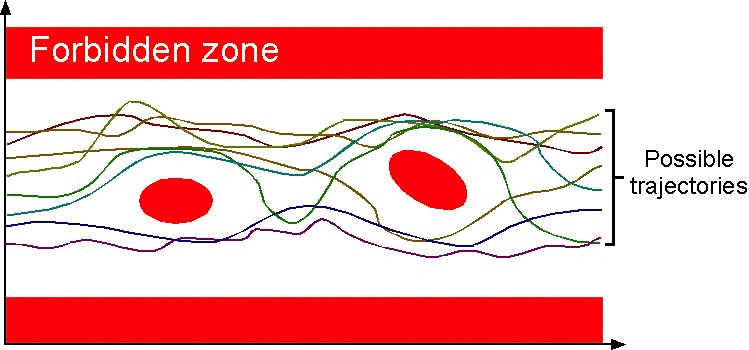
\includegraphics[width=1 \linewidth]{ai_1.png}
        \caption{
            \emph{Concrete semantics} of programs with
            \emph{forbidden zones}
        }
        \label{fig:ai1}
    \end{subfigure}
%
    \hfill
%
    \begin{subfigure}[hbt]{.45\linewidth}
        \centering
        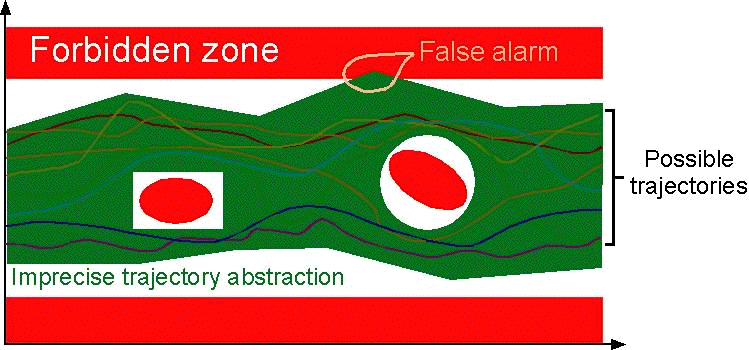
\includegraphics[width=1 \linewidth]{ai_2.png}
        \caption{
            \emph{Abstract semantics} of programs with imprecise
            trajectory abstraction
        }
        \label{fig:ai2}
    \end{subfigure}

    \caption{
        Abstract interpretation demonstration~\cite{AIInNutshellCousot}.
        Horizontal axes: time~$ t $. Vertical axes:
        vector~$ x(t) $~of input values of programs
    }
\end{figure}

\subsubsection*{Components of Abstract Interpretation}

In accordance with~\cite{favAI}, \cite{projectPracticeMarcin2018},
basic components of abstract interpretation are as follows:
\begin{itemize}
    \item \textbf{Abstract Domain}~\cite{AICousotWeb}
        \begin{itemize}
            \item
                An abstraction of the \emph{concrete semantics} in the form
                of \emph{abstract properties}\footnote{\textbf{Abstract
                properties} approximating \emph{concrete properties
                behaviours}.} and \emph{abstract
                operations}\footnote{\textbf{Abstract operations} include
                abstractions of the \emph{concrete approximation}, an
                approximation of the \emph{concrete fixpoint transform
                function}, etc.}.~\cite{AIBasedFormalMethodsCousot}

            \item
                Sets of program states at certain locations are represented
                using \emph{abstract states}.
        \end{itemize}

    \item \textbf{Abstract Transformers}
        \begin{itemize}
            \item
                There is a~\emph{transform function} for each program
                operation (instruction) that represents the impact
                of the operation executed on an abstract state.
        \end{itemize}

    \item \textbf{Join Operator}~$ \circ $
        \begin{itemize}
            \item
                Joins abstract states from individual program branches into
                a~single one.
        \end{itemize}

    \item
        \textbf{Widening
        Operator~$ \triangledown $}~\cite{programAnalysisNielson},
        \cite{wideningNarrowingCousot}, \cite{favAI}
        \begin{itemize}
            \item
                Enforces termination of the abstract interpretation.

            \item
                It is used to approximate the \emph{least fixed points}
                (it is performed on a~sequence of abstract states at
                a~certain location).

            \item
                The later in the analysis is this operator used, the more
                accurate is the result (but the analysis takes more time).
        \end{itemize}

    \item
        \textbf{Narrowing
        Operator~$ \vartriangle $}~\cite{programAnalysisNielson},
        \cite{wideningNarrowingCousot}, \cite{favAI}
        \begin{itemize}
            \item
                Encapsulates a~termination criterion.

            \item
                Using this operator, the approximation can be refined, i.e.,
                it may be used to refine the result of widening.

            \item
                This operator is used when a~\emph{fixpoint} is
                approximated using widening.
        \end{itemize}
\end{itemize}

\subsubsection*{Fixpoints and Fixpoint Approximation}

In~\cite{favLatticesAndFixpoints}, there is a~\emph{fixpoint} defined as:
\begin{itemize}
    \item
        let $ (A, \leq_A) $ be a~\emph{lattice}~\cite{favLatticesAndFixpoints},

    \item
        an element $ a \in A $ is a~\textbf{fixpoint} of a~function
        $ f : A \rightarrow A $ if and only if $ \boldsymbol{f(a) = a} $.
\end{itemize}
Computation of the \emph{most precise abstract fixpoint} is not generally
guaranteed to terminate in certain cases, such as loops. The solution is
to approximate the fixpoint using \emph{widening} (over-approximation of
a~fixpoint) and \emph{narrowing} (improves an approximation of
a~fixpoint)~\cite{favAI}, \cite{projectPracticeMarcin2018}.
Most program properties can be represented as fixpoints. This reduces a~program
analysis to the fixpoint approximation~\cite{AICousotWeb}. Further
information about fixpoint approximation can be found
in~\cite{programAnalysisNielson}, \cite{wideningNarrowingCousot}.

\subsubsection*{Formal Definition of Abstract Interpretation}

According to~\cite{AILatticeModelCousot}, \cite{favAI},
\textbf{abstract interpretation}~$ \boldsymbol{I} $~of a~program~$ P $~with
the instruction set~$ S $~is a~tuple
$$ \boldsymbol{I = (Q, \circ, \sqsubseteq, \top, \bot, \tau)} $$
where
\begin{itemize}
    \item
        $ \boldsymbol{Q} $~is the \emph{abstract domain} (domain of
        \emph{abstract states}),

    \item
        $ \boldsymbol{\circ}~\text{:}~Q \times Q \rightarrow Q $ is the \emph{join
        operator} for accumulation of abstract states,

    \item
        $ \text{(}\boldsymbol{\sqsubseteq}\text{)} \subseteq Q \times Q $ is an
        ordering defined as $ x \sqsubseteq y \Leftrightarrow x \circ y = y $ in
        $ (Q, \circ, \top) $,

    \item
        $ \boldsymbol{\top} \in Q $ is the \emph{supremum} of~$ Q $,

    \item
        $ \boldsymbol{\bot} \in Q $ is the \emph{infimum} of~$ Q $,

    \item
        $ \boldsymbol{\tau}~\text{:}~S \times Q \rightarrow Q $
        defines the \emph{abstract transformers} for specific instructions,

    \item
        $ (Q, \circ, \top) $ is a~\emph{complete
        semilattice}~\cite{favLatticesAndFixpoints}, \cite{favAI}.
\end{itemize}
Using so-called \emph{Galois connections}~(\cite{programAnalysisNielson},
\cite{wideningNarrowingCousot}, \cite{favAI}, \cite{AICousotWeb}) can be
guaranteed the \emph{soundness} of abstract interpretation.


\section{\texorpdfstring{Facebook Infer\,--\,Static Analysis Framework}{}}
\label{sec:fbinfer}

This section describes the principles and features of
\emph{Facebook Infer}. The description is based on information provided
on Facebook Infer website\footnote{\textbf{Facebook Infer}
website\,--\,\url{https://fbinfer.com}.} and in~\cite{inferAISlides},
\cite{projectPracticeMarcin2018}. Parts of this section are taken
over~\cite{excel2019FBInfer}.

\begin{figure}[hbt]
    \centering
    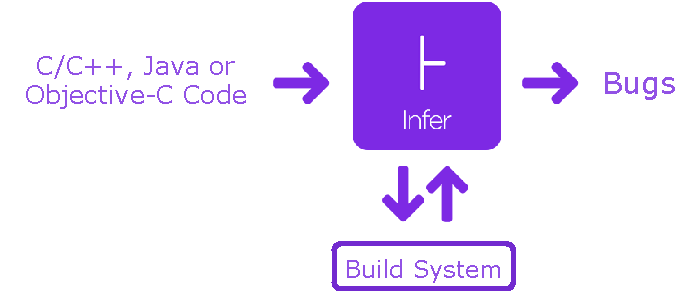
\includegraphics[width=.7 \linewidth]{infer.pdf}
    \caption{
        A~static analysis in Facebook Infer
        (\url{http://www.codeandyou.com/2015/06/infer-static-analyzer-for-java-c-and.html})
    }
    \label{fig:infer}
\end{figure}

Facebook Infer is an open-source static analysis \emph{framework},
which is able to discover various kinds of software bugs of a~given
program, and the stress is put on \emph{scalability}.
Elementary essence of this framework shows Figure~\ref{fig:infer}, below
is a~more detailed explanation of its architecture. Facebook Infer
itself is implemented in \emph{OCaml}\footnote{\textbf{OCaml}
website\,--\,\url{https://ocaml.org}.}\,--\,functional programming
language, also supporting imperative and object-oriented paradigms. Further
details about OCaml can be found in~\cite{realWorldOCaml} or in
official documentation\footnote{\textbf{OCaml
documentation}\,--\,\url{http://caml.inria.fr/pub/docs/manual-ocaml}.},
tutorials\footnote{\textbf{OCaml
tutorials}\,--\,\url{https://ocaml.org/learn/tutorials}.}. Facebook Infer was
originally a~standalone tool focused on \emph{sound verification} of
the absence of \emph{memory safety violations}, which has made its breakthrough
thanks to a~powerful paper~\cite{inferBiabduction}.

Facebook Infer is able to analyse programs written in several languages.
In particular, it supports languages C, C++, Java, and Objective-C. Moreover,
it is possible to extend Facebook Infer's \emph{frontend} for supporting
another languages. Currently, Facebook Infer contains many analyses focusing
on amount sorts of bugs, e.g., \emph{Inferbo} (buffer
overruns)~\cite{inferboOnline}; \emph{RacerD} (data races)~\cite{racerD},
\cite{racerDOnline}, \cite{staticRaceDetectorTruePositive}; \emph{RacerX}
(race conditions and deadlocks)~\cite{racerX}; and other analyses checks
for buffer overflows, thread-safety, null-dereferencing, memory leaks,
resource leaks, etc.


\subsection{Abstract Interpretation in Facebook Infer}

Facebook Infer is a~general framework for a~static analysis of programs, it is
based on \emph{abstract interpretation}, see Section~\ref{sec:AI}. It aims
to find bugs rather than formal verification. It can be used to quickly develop
new sorts of \emph{compositional} and \emph{incremental} analysers
(\emph{intraprocedural} or
\emph{interprocedural}~\cite{programAnalysisNielson}) based
on the concept of function \emph{summaries}. In general, a~\emph{summary}
is a~representation of \emph{preconditions} and \emph{postconditions} of
a~function. However, in practice, a~summary is a~custom data structure that
may be used for storing any information resulting from the analysis of
single functions. Facebook Infer generally does not work out the summaries
in the course of the analysis along the \emph{Control Flow Graph}
(\textbf{CFG})\footnote{\textbf{A~control flow graph (CFG)} is a~directed
graph in which the nodes represent basic blocks and the edges represent control flow paths.~\cite{controlFlowAnalysisAllen}} as it is done in classical analyses
based on the concepts from~\cite{dataflowAnalysisGraphReachability},
\cite{dataflowAnalysisApproaches}. Instead, Facebook Infer performs the
analysis of a~program \emph{function-by-function along the call tree},
starting from its leafs (demonstrated later). Therefore a~function
is analysed and a~summary is computed without knowledge of the
call context. Since summaries worked out in different contexts are equal,
this principle makes the analysis more scalable, but it can lead to
a~loss of accuracy. Then, the summary of a~function is used at all of its
call sites. In order to create new intraprocedural analyser in Facebook
Infer, it is needed to define (listed items are described in more detail
in Section~\ref{sec:AI}):
\begin{enumerate}
    \item
        An \emph{abstract domain}~$ Q $, i.e., the type of an
        \emph{abstract state}.

    \item
        Operator~$ \sqsubseteq $, i.e., an ordering of abstract states.

    \item
        \emph{Join} operator~$ \circ $, i.e., the way of joining two abstract
        states.

    \item
        \emph{Widening} operator~$ \triangledown $, i.e., the way how to
        enforce termination of the abstract interpretation of iteration.

    \item
        \emph{Transfer functions}~$ \tau $, i.e., a~transformer that
        takes an abstract state as input and produces an abstract state
        as output.
\end{enumerate}
And in order to create an interprocedural analyser, it is required to
additionally define:
\begin{enumerate}
    \item
        The type of function summaries.

    \item
        The logic for using summaries in transfer functions, and the logic
        for transforming an intraprocedural abstract state to
        a~summary.
\end{enumerate}
The next important feature improving the scalability is
\emph{incrementality} of the analysis, it allows to analyse separate
code changes only, instead of analysing the whole codebase. It is more
suitable for extensive and variable projects, where ordinary analysis
is not feasible. The incrementality is based on \emph{re-using summaries}
of functions for which there is no change in them neither in the functions
transitively invoked from them.

\subsubsection*{
    The Architecture of the Abstract Interpretation Framework in
    Facebook Infer
}

\begin{figure}[hbt]
    \centering
    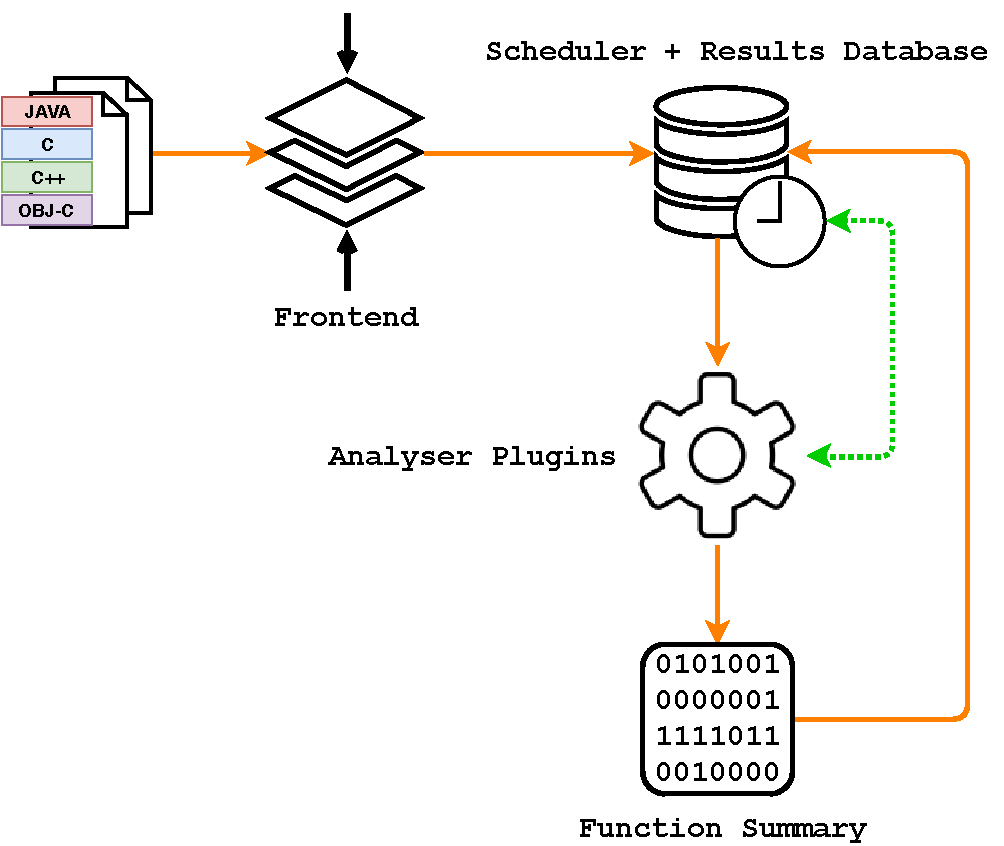
\includegraphics[width=.65 \linewidth]{infer_architecture.pdf}
    \caption{
        The architecture of Facebook Infer's abstract interpretation
        framework~\cite{inferAISlides}, \cite{projectPracticeMarcin2018}
    }
    \label{fig:inferArchitecture}
\end{figure}

The architecture of the abstract interpretation framework of Facebook
Infer (\textbf{Infer.AI}) may be split into three major parts,
as demonstrates Figure~\ref{fig:inferArchitecture}: a~\emph{frontend},
an \emph{analysis scheduler} (and a~\emph{results database}), and a~set of
\emph{analyser plugins}.

The frontend compiles input programs into the \emph{Smallfoot Intermediate
Language} (SIL) and represents them as the CFG. There is a~separate CFG
representation for each analysed function. Nodes of this CFG are formed as
instructions of SIL. SIL language consists of following underlying
instructions:
\begin{enumerate}
    \item
        \texttt{LOAD}\,--\,reading into a~temporary variable.

    \item
        \texttt{STORE}\,--\,writing to a~program variable,
        a~field of a~structure, or an array.

    \item
        \texttt{PRUNE~e}~(often called
        \texttt{ASSUME})\,--\,a~condition~\texttt{e}.

    \item
        \texttt{CALL}\,--\,a~function call.
\end{enumerate}
The frontend allows one to propose \emph{language-independent} analyses
(to a certain extent) because it supports input programs to be written
in multiple languages.

The next part of the architecture is the scheduler, which defines the
order of the analysis of single functions according to the appropriate
\emph{call graph}\footnote{\textbf{A~call graph} is \emph{directed graph}
describing call dependencies among functions.}. The scheduler also checks
\begin{wrapfigure}{r}{.45 \linewidth}
    \centering
    \vspace{-.5em}
    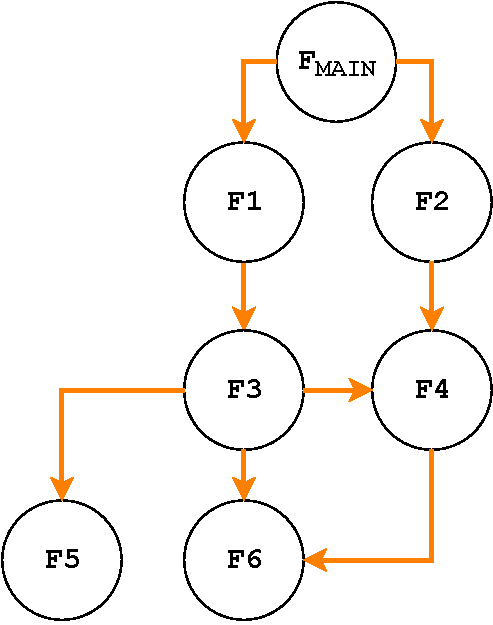
\includegraphics[width=.23 \textwidth]{infer_call_graph.pdf}
    \caption{
        A~call graph for an illustration of Facebook Infer's
        analysis process~\cite{inferAISlides}, \cite{excel2019FBInfer},
        \cite{projectPracticeMarcin2018}
    }
    \label{fig:inferCallGraph}
\end{wrapfigure}
if it is possible to analyse some functions simultaneously, which allows
Facebook Infer to run the analysis in parallel. For demonstrating the order
of the analysis in Facebook Infer and its incrementality, assume a~call
graph in Figure~\ref{fig:inferCallGraph}. At first, leaf functions
\texttt{P5} and \texttt{P6} are analysed. Further, the analysis goes on
towards the root of the call graph\,--\,\texttt{P\textsubscript{MAIN}},
while takes into consideration the dependencies denotes by the edges. This
order ensures that a~summary is available once a~nested function call is
abstractly interpreted within the analysis. When there is a~subsequent code
change, only directly changed functions and all the functions up the call
path are re-analysed. For instance, if there is a~change of source code of
function \texttt{P4}, Facebook Infer triggers re-analysation of functions
\texttt{P4}, \texttt{P2}, and \texttt{P\textsubscript{MAIN}} only.

The last part of the architecture consists of the set of analyser plugins.
Each plugin performs the analysis by interpretation of SIL instructions.
Result of the analysis of each function (function summary) is stored to
the results database. Interpretation of SIL instructions (\emph{commands})
is done using an \emph{abstract interpreter} (also called a~\emph{control
interpreter}) and \emph{transfer functions} (also called a~\emph{command
interpreter}). The transfer functions take an actual \emph{abstract state}
of an analysed function as input, and by applying the interpreting command
produce a~new abstract state. Then, the abstract interpreter interprets the
command in \emph{abstract domain} according to the CFG. This workflow is
simplified in Figure~\ref{fig:inferAnalysis}.

\begin{figure}[hbt]
    \centering
    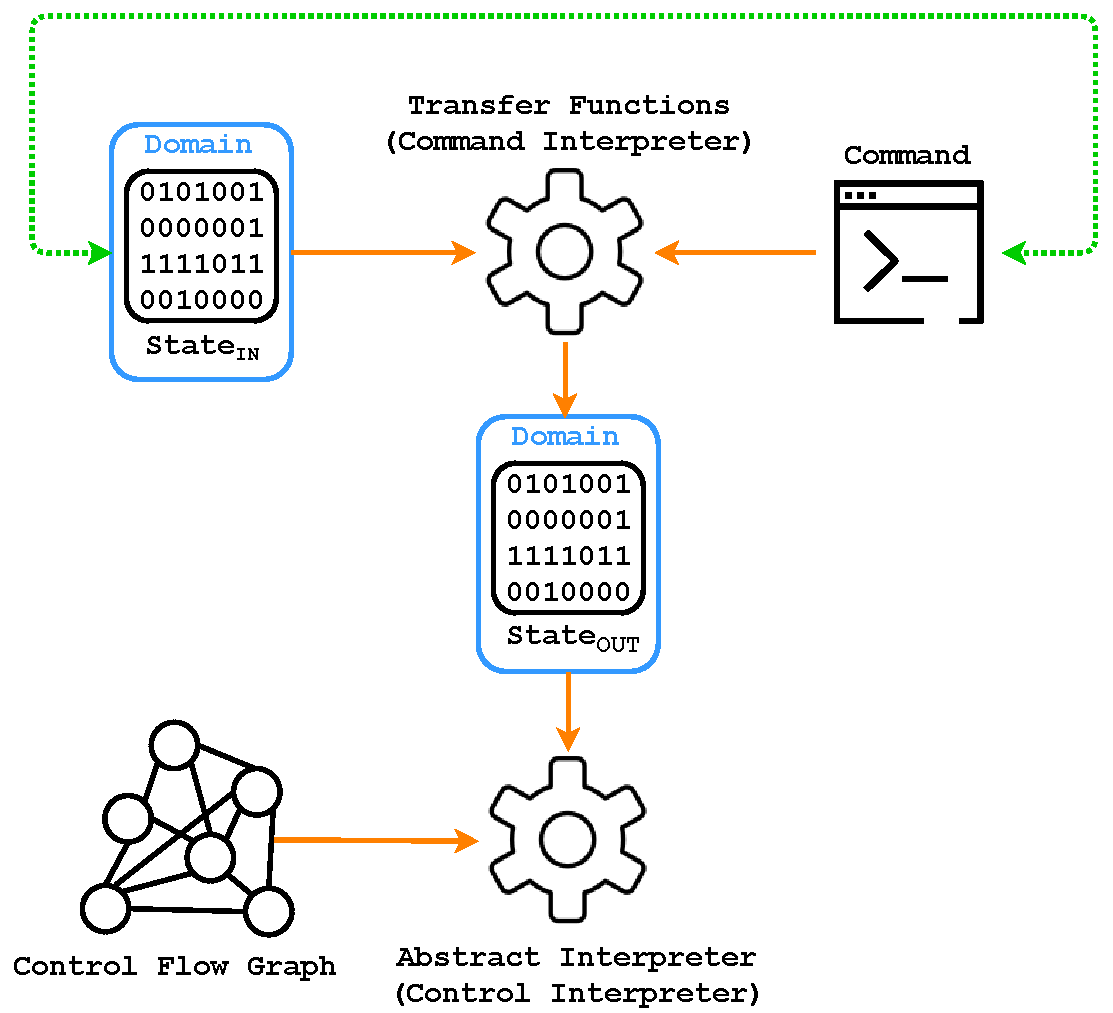
\includegraphics[width=.65 \linewidth]{infer_analysis.pdf}
    \caption{
        Facebook Infer's abstract interpretation
        process~\cite{inferAISlides}, \cite{projectPracticeMarcin2018}
    }
    \label{fig:inferAnalysis}
\end{figure}


\section{Contracts for Concurrency}
\label{sec:contracts}

This section introduces and defines the concept of \emph{contracts for
concurrency} described in~\cite{contracts2015}, \cite{contracts2017}. Parts
of this section are taken over~\cite{excel2019FBInfer}. Listings in this
section are pieces of programs written in ANSI~C\footnote{
\textbf{ANSI~C}\,--\,standard for the C~programming language published by
the \emph{ANSI} (American National Standards Institute).}.

Respecting the \emph{protocol} of a~software module\,---\,delineates
which sequences of functions are legal to invoke\,---\,is one of the
requirements for the correct behaviour of the module. For example, a~module
that deals with file system typically requires that the programmer using
this module should call function \texttt{open} at first, followed by an
arbitrary number of functions \texttt{read} and \texttt{write}, and at last,
call function \texttt{close}. A~program utilising such module that does
not follow this protocol is incorrect. The methodology of \emph{design by
contract} (described in~\cite{contract}) enforces programs to meet
such well-defined behaviours.~\cite{contracts2015}

In \emph{concurrent programs}, contracts for concurrency allow one to define
\emph{sequences of functions} that are required to be \emph{executed
atomically}, in order to avoid \emph{atomicity violations}. Such contracts
may be manually written by a~developer or it may be automatically generated
by a~program (analyser). These contracts can be used to verify the correctness
of programs as well as it can serve as useful documentation. A~program is
safe from \emph{atomicity violations} if the program respects a~contract and
the contract is well defined and complete.

Section~\ref{sec:basicContracts} defines the notion of \emph{basic contracts}
for concurrency. Further, Section~\ref{sec:parameterContracts} defines
contracts extended to reflect the \emph{data flow} between functions (i.e.,
a~sequence of function calls must be atomic only if they handle the
same data). Above that, paper~\cite{contracts2017} extends the notion
of basic contracts with \emph{spoilers} (i.e., extending by
\emph{contextual information}).


\subsection{Basic Contracts}
\label{sec:basicContracts}

In~\cite{contracts2017}, \cite{contracts2015}, a~\emph{basic contract} is
formally defined as follows. Let~$ \Sigma_\mathbb{M} $~be a~set of all
function names of a~software module. A~contract is
a~set~$ \mathbb{R} $~of \emph{clauses} where each clause
$ \varrho\ \in \mathbb{R} $ is a~\emph{star-free regular
expression}\footnote{\textbf{Star-free regular expressions} are
regular expressions using only the \emph{concatenation operators}
and \emph{alternative operators} ($ | $), without the
\emph{Kleene star operator} ($ * $).} over~$ \Sigma_\mathbb{M} $.
A~\emph{contract violation} occurs if any of the sequences represented by
the contract clauses is interleaved with an execution of functions
from~$ \Sigma_\mathbb{M} $, in other words, each sequence defined by
any clause~$ \varrho $~must be executed atomically, otherwise there
is a~violation of the contract. The number of sequences specified by
the contract is finite, because the contract is the union of
\emph{star-free languages}.

Consider the following example from~\cite{contracts2017}. There is
a~module with implementation of a~resizable array with the following
functions:
\begin{itemize}[label=]
    \tt

    \item void add(char *array, char element)
    \item bool contains(char *array, char element)
    \item int index\_of(char *array, char element)
    \item char get(char *array, int index)
    \item void set(char *array, int index, char element)
    \item void remove(char *array, int index)
    \item int size(char *array)
\end{itemize}
The module contains following clauses:
\begin{enumerate}[label={$ (\varrho_{\arabic*}) $}]
    \item
        \texttt{contains index\_of}
        \begin{itemize}
            \item
                Execution of \texttt{contains} followed by \texttt{index\_of}
                should be atomic. Otherwise, the program may failed to
                get the index, because after confirmation of its existence
                in an array, it can be concurrently, e.g., removed.
        \end{itemize}

    \item
        \texttt{index\_of (get | set | remove)}
        \begin{itemize}
            \item
                Execution of \texttt{index\_of} follow by \texttt{get},
                \texttt{set}, or \texttt{remove} should be atomic. Otherwise,
                the obtained index may be outdated when it is used to access
                an element, because a~concurrent change of an array may shift
                the position of the element.
        \end{itemize}

    \item
        \texttt{size (get | set | remove)}
        \begin{itemize}
            \item
                Execution of \texttt{size} follow by \texttt{get},
                \texttt{set}, or \texttt{remove} should be atomic. Otherwise,
                the size of an array may be invalid when accessing an array,
                because of a~concurrent change of the array. This can be
                in issue, since a~given index is not in valid range
                anymore (e.g., \texttt{index < size}).
        \end{itemize}

    \item
        \texttt{add (get | index\_of)}
        \begin{itemize}
            \item
                Execution of \texttt{add} followed by \texttt{get} or
                \texttt{index\_of} should be atomic. Otherwise, the added
                element may no longer exists or its position in an array
                may be changed, when the program tries to get information
                about it.
        \end{itemize}
\end{enumerate}

The above definition of contracts for concurrency is quite limited in
some cases and can consider valid concurrent programs as incorrect (reports
\emph{false alarms}). Hence, in Section~\ref{sec:parameterContracts},
there is defined an extension with \emph{parameters}, which considering the
data flow between function calls. And in~\cite{contracts2017}, there
is defined another extension with \emph{spoilers}, which considering
contextual information of function function calls.


\subsection{Contracts with Parameters}
\label{sec:parameterContracts}

\begin{lstlisting}[
    style=c, label={list:contractsReplace}, float=hbt,
    caption={
        An example of an atomicity violation with data
        dependencies~\cite{contracts2017}
    }
]
void replace(char *array, char a, char b)
{
    if (contains(array, a))
    {
        int index = index_of(array, a);
        set(array, index, b);
    }
}
\end{lstlisting}

Consider the following example from~\cite{contracts2017}, as demonstrates
Listing~\ref{list:contractsReplace}. There is a~function \texttt{replace}
that replaces item~\texttt{a}~in an array by item~\texttt{b}. Implementation
of this function contains two atomicity violations:
\begin{enumerate}[label={(\roman*)}]
    \item
        item~\texttt{a}~does not need to exist anymore when \texttt{index\_of}
        is called,

    \item
        the index acquired can be obsolete when \texttt{set} is called.
\end{enumerate}
A~basic contract from Section~\ref{sec:basicContracts} could cover
this scenario by a clause:
$$ (\varrho_5)\ \text{\texttt{contains index\_of set}} $$
However, it is too restrictive because it is required to be executed
atomically only if \texttt{contains} and \texttt{index\_of} have the same
arguments \texttt{array} and \texttt{element}, \texttt{index\_of} and
\texttt{set} have the same arguments \texttt{array}, and the returned value of
\texttt{index\_of} is used as the argument \texttt{index} of function
\texttt{set}.

In order to consider \emph{function call parameters} and \emph{return values}
of functions in contracts, the basic contracts are extended by dependencies
between functions in~\cite{contracts2017} as follows. Function call parameters
and return values are expressed as \emph{meta-variables}. Further, if a~contract
should be enforced only if the same object appears as an argument or as
the return value of multiple calls in a~given call sequence, it can be expressed
by using the same meta-variable at the position of all these parameters
and/or return values.

Clause~$ \varrho_5 $~can be extended as follows (repeated use of
meta-variables \texttt{X/Y/Z} requiring to appear the same objects
\texttt{o\textsubscript{1}/o\textsubscript{2}/o\textsubscript{3}} at the
positions of \texttt{X/Y/Z}).
$$
    (\varrho^\prime_5)\ \text{\texttt{
        contains(X,Y) Z=index\_of(X,Y) set(X,Z,\_))
    }}
$$
The underscore means a \emph{free meta-variable} that does not restrict
the the contract clause.

With this extension, it is possible to extend contract from
Section~\ref{sec:basicContracts} as follows:
\begin{enumerate}[label={$ (\varrho^\prime_{\arabic*}) $}]
    \tt

    \item contains(X,Y) index\_of(X,Y)
    \item Y=index\_of(X,\_) (get(X,Y) | set(X,Y,\_) | remove(X,Y))
    \item Y=size(X) (get(X,Y) | set(X,Y,\_) | remove(X,Y))
    \item add(X,Y) (get(X,Y) | index\_of(X,Y))
\end{enumerate}



\chapter{Proposal of Static Analyser for Detecting Atomicity Violations}
\label{chap:proposal}



\chapter{Implementation of the Analyser in Facebook Infer}
\label{chap:implementation}



\chapter{Experimental Verification and Evaluation of the Analyser}
\label{chap:experiments}



\chapter{Conclusion}
\label{chap:conclusion}


%===============================================================================
